\documentclass[border=4pt]{standalone}

% --- packages (mirror these in embedding.meta.json "requires") ---
\usepackage{tikz}

% --- palette (canonical source: reference/color-palettes/color-palettes.md; light variant) ---
\definecolor{otblue}{HTML}{0072B2}
\definecolor{otorange}{HTML}{E69F00}
\definecolor{otteal}{HTML}{009E73}
\definecolor{otpurple}{HTML}{CC79A7}
\definecolor{otgray}{HTML}{5A5A5A}

\begin{document}
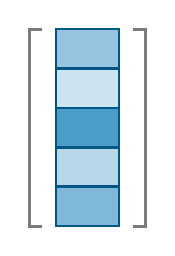
\begin{tikzpicture}[line width=0.9pt]
  % embedding vector: a column of weighted cells
  \foreach \i/\c in {0/otblue!50, 1/otblue!28, 2/otblue!70, 3/otblue!20, 4/otblue!42}{
    \filldraw[draw=otblue!75!black, fill=\c] (0,\i*0.5) rectangle (0.8,\i*0.5+0.5);
  }
  % vector brackets
  \draw[otgray!80, line width=1.1pt] (-0.18,0) -- (-0.34,0) -- (-0.34,2.5) -- (-0.18,2.5);
  \draw[otgray!80, line width=1.1pt] (0.98,0) -- (1.14,0) -- (1.14,2.5) -- (0.98,2.5);
\end{tikzpicture}
\end{document}
